\chapter{Architecture et description du logiciel}
Cette section concerne la description de l'architecture du projet, en abordant tout d'abord le parsing, puis l'analyse des données et le rendu graphique.

%Dans cette partie, nous allons d'abord vous parler de la partie concernant le parsing puis passer à la partie d'analyse des données et de rendu graphique.

\section{Architecture globale}

\begin{figure}[!h]
  \begin{center}
    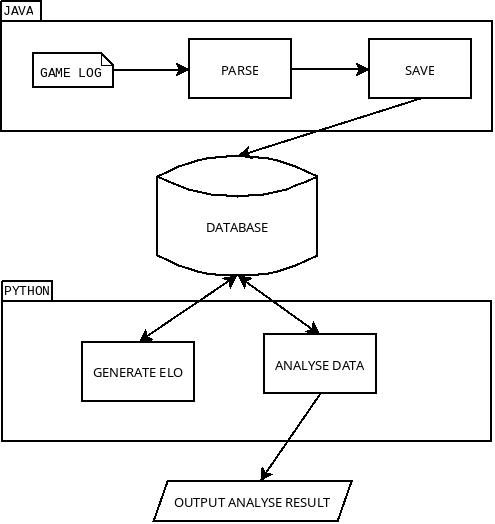
\includegraphics[scale=0.45, keepaspectratio]{./presentation/overview.jpg}
  \end{center}
  \caption{représentation de l'architecture globale du projet}
\end{figure}

L'architecture du projet se décompose en 3 parties distinctes et indépendantes. Un premier élément, développé en Java, est responsable du parsing destiné à analyser et structurer les données, dans un format compatible avec la base de données, et de s'en servir pour l'alimenter.\\

%charger les données e première partie permet de charger les données contenues dans les Logs puis de les inscrire dans la base de données.\newline
La base de données stocke ces données et peut en recevoir de nouvelles ou bien répondre aux requetes qui lui sont soumises.\\

La dernière partie correspond à une bibliothèque en Python qui met à disposition des outils permettant de raffiner et d'analyser les données disponibles dans la base. \\

%permettant à l'utilisateur d'effectuer des analyses prédéfinies ou bien de produire ses propres analyses. Pour cela, l'utilisateur dispose de fonctions de communications avec la base de données.

\section{Parser}
%Cette partie est écrite en java, l'autre possibilité que nous avions était de coder le parser en python mais après quelques petits tests nous nous sommes rendus compte que le parser en python serait beaucoup trop lent. Voici l'architecture de la partie Java de notre projet:
\begin{figure}[!h]
  \begin{center}
    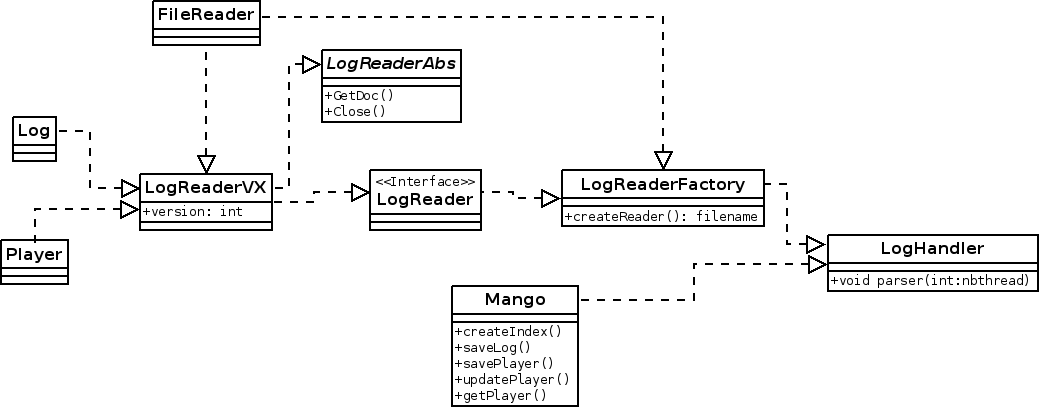
\includegraphics[width=\textwidth,height=\textheight,keepaspectratio]{diaRessources/nouvelleArch}
  \end{center}
  \caption{Représentation de l'architecture de la partie parser}
\end{figure}
En raison d'évolutions constantes du serveur du jeu, les formats des \textit{Logs} présentent de petites différences. Plusieurs tranches de \textit{Logs} existent, qui traduisent les changements apportés aux formats au fil du temps. 
Pour résoudre ce problème il a fallu identifier les tranches, leur donner un numéro de version, et créer un \textit{LogReader} adapté à chaque version. A cette fin, il a été utilisé un \textit{design pattern factory}.
Pour la création des \textit{LogReaders}, une classe abstraite, la \textit{LogReaderAbs} a été créée, comportant toutes les méthodes utilisées pour le parsing qui sont communes à l'ensemble des \textit{LogReaders}. 

%En raison de logs au format variable, il est nécessaire de produire plusieurs versions de parser afin de garder une robustesse au niveau du parsing et d'éviter une classe trop grosse. Pour cela, à l'ouverture d'un log, le LogHandler demande la création d'un parser à une classe utilisant le design pattern factory. Cette classe va examiner le log en question et choisir la bonne version du parser a utiliser puis renvoyer ce parser au log handler. Afin d'éviter des duplications de code inutiles, le parser en lui même est implémenté à l'aide d'une classe abstraite regroupant toutes les similitudes entre les parsers puis les différences sont implémentées dans la classe du parser en question à proprement parler. Le LogHandler va ensuite envoyer sur une base de données les données obtenues à l'aide du parser.
La classe \textit{LogHandler} est chargée de demander au \textit{LogReaderFactory} la création d'un \textit{LogReader} correspondant à la version à traiter et de demander au parser de générer les documents puis de les envoyer à la base de données. 
 
\section{Base de données}
MongoDB a été choisi pour gérer les documents ainsi générés car ses caractéristiques correspondent aux besoins du projet : quantité volumineuse de données, grande vitesse de recherche, format des données adapté. 
%L'implémentation de la base de données retenue est MongoDB, nous l'avons retenue du fait qu'elle soit orientée documents et du fait qu'elle autorise une compression des données stockées. Elle communique avec le parser ainsi que la librairie proposée à l'utilisateur.\\
%Elle est capable de recevoir de nouvelles données à stocker, de modifier sa structure (changement ou ajout de champs dans les données) et modifier les données contenues.

\section{Bibliothèque}
Cette partie est écrite en Python à la demande du client. Plusieurs bibliothèques, contenant des outils nécessaires pour travailler sur les données acquises lors du parsing, sont proposées. Il s'agira de la structure des données, de l'interface de communication avec la base de données, et d'outils utilisables par le client.

Voici un schéma regroupant les différents modules et leurs liens:
\begin{figure}[!h]
  \begin{center}
    \includegraphics[width=\textwidth,height=\textheight,keepaspectratio]{diaRessources/Python_arch}\\
  \end{center}
  \caption{Représentation de l'architecture de la partie Analyse des données}
\end{figure}

\subsection{Structure des données}
Il s'agissait de créer des structures de données facilitant le travail à effectuer sur celles-ci. Un type de données est appelé \textit{Match} ; il correspond aux documents "Log" ; un autre type est dénommé \textit{SimplifiedPlayer}, et correspond aux données concernant les joueurs et leur ELO final. 


%Tout d'abord, le module MongoInterface permet de communiquer avec la base de données.\newline
%Les objets Matchs et Player sont utilisés lors de la récupération de données afin de les mettre en forme pour une utilisation plus aisée par le client. Ce sont des structures de données regroupant toutes les information relatives au match ou joueur en question.\newline
%La bilbiothèque Tools regroupe les fonctions d'analyse basique pouvant être utilisées sur les logs, pour appliquer ces fonctions, il faut utiliser la fonction \textit{apply\_function\_to\_query}. Si dans le futur, le client ou bien des personnes souhaitant travailler sur ce projet veulent étoffer les fonctions proposées, il suffira de les ajouter dans cette libraire.\newline
%La solution proposée pour afficher les resultats consiste en un module Plotter et un module DataSet. Le module DataSet permet de mettre en forme les données à représenter de manière simple pour l'utilisateur, et le module Plotter propose une solution simple pour afficher des résultats de base (lignes cassées, nuage de points ou barres).

\subsection{Interface de communication avec la base de données}
Cette interface a été créée pour faciliter la communication du client avec la base de données :elle comprend des outils comme la récupération de documents, la recherche de "logs", la recherche de joueurs. Le nom de ce module est \textit{MongoInterface}.

\subsection{Outils}
Il s'agit d'un ensemble de fonctions destinées à raffiner et analyser les données de la base. On y trouve les fonctionnalités suivantes : 
\begin{itemize}
\item génération de \textit{SimplifiedPlayers} dans la base de données
\item calcul d'ELO pour chaque \textit{SimplifiedPlayers} et chaque \textit{Log}
\item génération de courbes d'ELO pour un joueur donné
\item génération de listes contenant les \textit{greenings} pour chague \textit{Log} de la base de données
\item tentative de reconnaissance des stratégies \textit{BigMoney} dans les \textit{Logs} (outil non fonctionnel)
\end{itemize}

\section{Extensions possibles}
Le projet étant arrivé à la phase où on pourrait commencer à exploiter les données, de nombreuses extensions sont certainement possibles. Dans l'état actuel des choses, il n'est malheureusement pas possible de les évoquer avec précision. 

%Sur la partie parser, il est très facile d'ajouter une nouvelle version de parser permettant de lire par exemple des logs d'un nouvelle version du serveur de jeu, cela permettrait de regouper des données sur une plus grande période et donc d'obtenir des statistiques plus intéressantes.\newline
%ur la partie Python, il est possible d'ajouter de nouvelles fonctions d'analyse des données, des données peuvent également être rajoutées pour les logs mais il faudra faire attention à la lecture de ces données car les objets ne permettrons pas un accès facile à celles-ci (sauf si l'utilisateur modifie également les structures de données).
